\hypertarget{a00846}{}\section{Known Issues}
\label{a00846}\index{Known Issues@{Known Issues}}
A list of known bugs affecting A\+AX plug-\/ins. 

\hypertarget{a00846_knownissues_contents}{}\subsection{Contents}\label{a00846_knownissues_contents}
\begin{DoxyItemize}
\item \mbox{\hyperlink{a00846_knownissues_aaxsdk}{Known Issues in the A\+AX S\+DK}} \item \mbox{\hyperlink{a00846_knownissues_ptsw}{Known Issues in Pro Tools}} \item \mbox{\hyperlink{a00846_knownissues_venue}{Known Issues in Venue Live Sound Systems}} \item \mbox{\hyperlink{a00846_knownissues_mc}{Known Issues in Media Composer}} \item \mbox{\hyperlink{a00846_knownissues_cs}{Known Issues in Control Surfaces}} \item \mbox{\hyperlink{a00846_knownissues_other}{Known Issues in Other Software}} \item \mbox{\hyperlink{a00846_knownissues_tools}{Known Issues in A\+AX Tools}}\end{DoxyItemize}
\hypertarget{a00846_knownissues_aaxsdk}{}\subsection{Known Issues in the A\+A\+X S\+DK}\label{a00846_knownissues_aaxsdk}
\hypertarget{a00846_AAXSDK-663}{}\subsubsection{A\+A\+X\+S\+D\+K-\/663}\label{a00846_AAXSDK-663}
A\+AX S\+DK {\ttfamily \#pragma pack} errors with X\+Code 10 and later

Resolution\+: This bug is fixed as of A\+AX S\+DK 2.\+3.\+2\hypertarget{a00846_AAXSDK-599}{}\subsubsection{A\+A\+X\+S\+D\+K-\/599}\label{a00846_AAXSDK-599}
In the Win32 G\+UI example plug-\/in, the mouse cursor disappears when text is entered in text box and only re-\/appears when the mouse is moved out of the plug-\/in window bounds

Resolution\+: This bug is unresolved\hypertarget{a00846_AAXSDK-561}{}\subsubsection{A\+A\+X\+S\+D\+K-\/561}\label{a00846_AAXSDK-561}
An A\+AX Hybrid D\+SP plug-\/in with 7.\+1.\+2 input and output stem formats and a 16-\/sample processing buffer size will throw an A\+AE -\/14382 error upon instantiation at 192k\+Hz

Resolution\+: This bug is unresolved\hypertarget{a00846_AAXSDK-533}{}\subsubsection{A\+A\+X\+S\+D\+K-\/533}\label{a00846_AAXSDK-533}
A\+A\+X\+Library compiles with warnings in Visual Studio 2015

Resolution\+: This bug is fixed as of A\+AX S\+DK 2.\+3.\+0\hypertarget{a00846_AAXSDK-514}{}\subsubsection{A\+A\+X\+S\+D\+K-\/514}\label{a00846_AAXSDK-514}
Using collection-\/level properties leads to a leaked A\+CF object

Resolution\+: This bug is fixed as of A\+AX S\+DK 2.\+3.\+0\hypertarget{a00846_AAXSDK-321}{}\subsubsection{A\+A\+X\+S\+D\+K-\/321}\label{a00846_AAXSDK-321}
Demo Delay (mono) D\+SP / Demo Gain (Cocoa UI) (mono) D\+SP can\textquotesingle{}t be instantiated

Resolution\+: This bug is fixed as of A\+AX S\+DK 2.\+2.\+0\hypertarget{a00846_AAXSDK-271}{}\subsubsection{A\+A\+X\+S\+D\+K-\/271}\label{a00846_AAXSDK-271}
Demo\+M\+I\+D\+I\+\_\+\+Sampler\+: No audio on right channel (multi-\/mono)

Resolution\+: This bug is fixed as of A\+AX S\+DK 2.\+2.\+0

Discussion\+: Demo\+M\+I\+D\+I\+\_\+\+Sampler and Demo\+M\+I\+D\+I\+\_\+\+Synth are now restricted to not use multi-\/mono, via the \mbox{\hyperlink{a00662_a13e384f22825afd3db6d68395b79ce0da83f671685958bdc668ef574d5a2d92b0}{A\+A\+X\+\_\+e\+Property\+\_\+\+Constraint\+\_\+\+Multi\+Mono\+Support}} property.

In Pro Tools, when a track\textquotesingle{}s M\+I\+DI destination is set to \char`\"{}none\char`\"{} and a new plug-\/in that includes a M\+I\+DI input node (e.\+g. any Instrument plug-\/in) is instantiated, the track\textquotesingle{}s M\+I\+DI destination is set to the first newly created M\+I\+DI input node.

When the track in question is greater than mono, and the Instrument plug-\/in is multi-\/mono, the default behavior is for the track\textquotesingle{}s M\+I\+DI destination to be set to the first of the newly created input nodes, not to all of them simultaneously. As a result, the track\textquotesingle{}s M\+I\+DI destination is set to the M\+I\+DI input node of the first (left) multi-\/mono instance of the plug-\/in.

To route M\+I\+DI to all channels of a multi-\/mono plug-\/in in Pro Tools, ctrl-\/select the M\+I\+DI destination and choose the additional M\+I\+DI nodes.\hypertarget{a00846_AAXSDK-186}{}\subsubsection{A\+A\+X\+S\+D\+K-\/186}\label{a00846_AAXSDK-186}
C99\+Compatibility constructs are incorrect when used with V\+S2012

Resolution\+: This bug is fixed as of A\+AX S\+DK 2.\+1.\+1\hypertarget{a00846_AAXSDK-162}{}\subsubsection{A\+A\+X\+S\+D\+K-\/162}\label{a00846_AAXSDK-162}
Misleading warning message when attempting hardware debugging using a non-\/local T\+I\+Shell.\+out

The \char`\"{}\+Load Pro\+Tools Plug-\/in Symbols\char`\"{} script gives the following warning\+: {\ttfamily D\+:/\+Code\+\_\+7/dev.ws.\+backup-\/win7-\/concert/\+A\+A\+X/\+Internal/\+System\+Software/\+T\+I\+Shell/\+C\+C\+S\+\_\+\+Project/\+T\+I\+Shell/../../../../../../\+Win\+Bag/x64/\+Release/bin/\+T\+I\+Shell.out does not exist! Please question everything.}

This error message includes a hard-\/coded path that is not relevant to the running system. This error is benign but it can be confusing.

Resolution\+: This bug is unresolved\hypertarget{a00846_AAXSDK-16}{}\subsubsection{A\+A\+X\+S\+D\+K-\/16}\label{a00846_AAXSDK-16}
A\+AX S\+DK\+: Win32 example plug-\/in G\+UI does not appear in Windows 8

Resolution\+: This bug is fixed as of A\+AX S\+DK 2.\+2.\+0\hypertarget{a00846_AAXSDK-14}{}\subsubsection{A\+A\+X\+S\+D\+K-\/14}\label{a00846_AAXSDK-14}
A\+AX Demo\+Gain\+\_\+\+V\+ST\+: Text box entry is not acknowledged upon click outside of window

Resolution\+: This bug is unresolved\hypertarget{a00846_AAXSDK-13}{}\subsubsection{A\+A\+X\+S\+D\+K-\/13 / A\+A\+X-\/579 / P\+T\+S\+W-\/158381}\label{a00846_AAXSDK-13}
A\+AX S\+DK Win32 example plug-\/in does not \char`\"{}snap to default\char`\"{} on option-\/click

Resolution\+: This bug is fixed as of A\+AX S\+DK 2.\+2.\+0\hypertarget{a00846_AAXSDK-11}{}\subsubsection{A\+A\+X\+S\+D\+K-\/11 / A\+A\+X-\/581 / P\+T\+S\+W-\/158348}\label{a00846_AAXSDK-11}
A\+AX S\+DK V\+S\+T\+G\+UI example plug-\/in does not respond to \textquotesingle{}alt\textquotesingle{} or \textquotesingle{}win\textquotesingle{} modifier keys (Windows)

Resolution\+: This bug is fixed as of A\+AX S\+DK 2.\+2.\+0\hypertarget{a00846_AAXSDK-10}{}\subsubsection{A\+A\+X\+S\+D\+K-\/10 / A\+A\+X-\/580 / P\+T\+S\+W-\/154083}\label{a00846_AAXSDK-10}
A\+AX Demo\+Gain\+\_\+\+V\+ST and Demo\+Gain\+\_\+\+Cocoa require initial click on G\+UI to take focus before editing (OS X)

Resolution\+: This bug is not yet resolved. For OS X, one workaround is to modify V\+S\+T\+G\+UI\textquotesingle{}s cocoasupport.\+mm file in order to add a handler for the accepts\+First\+Mouse selector\+:


\begin{DoxyCode}{0}
\DoxyCodeLine{\textcolor{keyword}{static} BOOL VSTGUI\_NSView\_acceptsFirstMouse(}
\DoxyCodeLine{  \textcolor{keywordtype}{id} \textcolor{keyword}{self},}
\DoxyCodeLine{  \textcolor{keywordtype}{SEL} \_cmd)}
\DoxyCodeLine{\{}
\DoxyCodeLine{  \textcolor{keywordflow}{return} YES;}
\DoxyCodeLine{\}}
\DoxyCodeLine{}
\DoxyCodeLine{\textcolor{comment}{// In VSTGUI\_NSView\_isOpaque()}}
\DoxyCodeLine{res = class\_addMethod(}
\DoxyCodeLine{  viewClass,}
\DoxyCodeLine{  \textcolor{keyword}{@selector}(acceptsFirstMouse:),}
\DoxyCodeLine{  IMP (VSTGUI\_NSView\_acceptsFirstMouse),}
\DoxyCodeLine{  \textcolor{stringliteral}{"B@:@:"});}
\end{DoxyCode}


Special thanks to Nick Protokowicz for suggesting this workaround.\hypertarget{a00846_AAXSDK-6}{}\subsubsection{A\+A\+X\+S\+D\+K-\/6 / A\+A\+X-\/646}\label{a00846_AAXSDK-6}
A\+AX S\+DK\+: Incorrect output from scatter/gather D\+MA example plug-\/in when increasing playback buffer size while audio is present (Native decks)

Resolution\+: This bug is unresolved

Workaround\+: The workaround for this issue is to not run audio through this plug-\/in while increasing the playback buffer size.\hypertarget{a00846_AAXSDK-5}{}\subsubsection{A\+A\+X\+S\+D\+K-\/5}\label{a00846_AAXSDK-5}
\mbox{\hyperlink{a01461_a25fc41a1060445db4d7bee7a2919460d}{A\+A\+X\+\_\+\+C\+Chunk\+Data\+Parser\+::\+Load\+Chunk}} doesn\textquotesingle{}t handle unknown chunk items well

Resolution\+: This bug will not be fixed

Discussion\+: \mbox{\hyperlink{a01461}{A\+A\+X\+\_\+\+C\+Chunk\+Data\+Parser}} does not store the size of each chunk item in the data stream. Therefore there is no way to determine the correct size for each data element when reading a chunk that was generated by this parser.

Workaround\+: If you know the correct size of each data element in a chunk when it is read by the plug-\/in, you can override the \mbox{\hyperlink{a01461}{A\+A\+X\+\_\+\+C\+Chunk\+Data\+Parser}} methods to ensure that each data element is correctly sized.\hypertarget{a00846_AAXSDK-2}{}\subsubsection{A\+A\+X\+S\+D\+K-\/2 / A\+A\+X-\/648}\label{a00846_AAXSDK-2}
A\+AX S\+DK\+: Output from D\+MA example plug-\/in is one buffer early

Resolution\+: This bug is unresolved\hypertarget{a00846_AAX-582}{}\subsubsection{A\+A\+X-\/582 / P\+T\+S\+W-\/157726}\label{a00846_AAX-582}
A\+AX S\+DK example plug-\/ins\textquotesingle{} controls do not write automation properly when in \textquotesingle{}touch\textquotesingle{} mode (frequently revert to default value while writing)

Resolution\+: This bug is fixed as of the 1.\+0.\+4 S\+DK\hypertarget{a00846_AAX-585}{}\subsubsection{A\+A\+X-\/585 / P\+T\+S\+W-\/157451}\label{a00846_AAX-585}
A\+AX Demo\+Gain G\+UI example plug-\/ins do not correctly handle alt/opt-\/click for resetting controls to their default state

Resolution\+: This bug is partially resolved as of A\+AX S\+DK 1.\+0.\+4. See also P\+T\+S\+W-\/158348 and P\+T\+S\+W-\/158381.\hypertarget{a00846_AAX-578}{}\subsubsection{A\+A\+X-\/578 / P\+T\+S\+W-\/158310}\label{a00846_AAX-578}
A\+AX S\+DK J\+U\+CE example plug-\/in does not \char`\"{}snap to default\char`\"{} on option-\/click

Resolution\+: This bug is fixed as of A\+AX S\+DK 1.\+0.\+4\hypertarget{a00846_knownissues_ptsw}{}\subsection{Known Issues in Pro Tools}\label{a00846_knownissues_ptsw}
\hypertarget{a00846_PT-250751}{}\subsubsection{P\+T-\/250751}\label{a00846_PT-250751}
Audio\+Suite plug-\/ins do not set a \mbox{\hyperlink{a01697_a60a29fda8490f240ecf869ff14fabf0e}{custom suffix}} on a clip in case the selection reference is \char`\"{}\+Clips list\char`\"{}

Resolution\+: This bug is unresolved\hypertarget{a00846_PT-249791}{}\subsubsection{P\+T-\/249791}\label{a00846_PT-249791}
Audio\+Suite\+: \mbox{\hyperlink{a01697_a60a29fda8490f240ecf869ff14fabf0e}{Custom clip name}} is not applied to generated audio file on disk

Resolution\+: This bug is unresolved\hypertarget{a00846_PT-249790}{}\subsubsection{P\+T-\/249790}\label{a00846_PT-249790}
Audio\+Suite plug-\/ins cannot set a \mbox{\hyperlink{a01697_a60a29fda8490f240ecf869ff14fabf0e}{custom clip name suffix}}

Resolution\+: This bug will be fixed in a Pro Tools 2019 release\hypertarget{a00846_PT-248000}{}\subsubsection{P\+T-\/248000}\label{a00846_PT-248000}
Plug-\/in partial bypass should support more than just EQ and Dynamics categories

Resolution\+: This enhancement is not yet supported\hypertarget{a00846_PT-245693}{}\subsubsection{P\+T-\/245693}\label{a00846_PT-245693}
Dynamic plug-\/in processing on H\+DX cuts off reverb tails

Resolution\+: This bug is unresolved\hypertarget{a00846_PT-243211}{}\subsubsection{P\+T-\/243211}\label{a00846_PT-243211}
Crash when closing a plug-\/in window unless the plug-\/in leaks its \mbox{\hyperlink{a01889}{A\+A\+X\+\_\+\+I\+View\+Container}} reference counts

Resolution\+: This bug is fixed as of Pro Tools 2019.\+5\hypertarget{a00846_PT-237857}{}\subsubsection{P\+T-\/237857}\label{a00846_PT-237857}
Custom EQ curve display ranges are not supported

Resolution\+: This enhancement is not yet supported\hypertarget{a00846_PT-236755}{}\subsubsection{P\+T-\/236755}\label{a00846_PT-236755}
Up-\/mixing plug-\/ins with A\+OS drop output channels on H\+DX

Resolution\+: This bug is fixed as of Pro Tools 2018.\+7\hypertarget{a00846_PT-235831}{}\subsubsection{P\+T-\/235831}\label{a00846_PT-235831}
The plug-\/in frame overlaps the plug-\/in window header if the plug-\/in G\+UI is taller than the screen height less the plug-\/in window header height.

Resolution\+: This bug is unresolved

Workaround\+: Avoid resizing the plug-\/in G\+UI to a height greater than the display height.\hypertarget{a00846_PT-235333}{}\subsubsection{P\+T-\/235333}\label{a00846_PT-235333}
Dynamic plug-\/in processing incorrectly shuts off processing in mixed multi-\/mono/multichannel chains that should force processing

This bug can occur if a multi-\/mono plug-\/in preceeds a multichannel plug-\/in which sets \mbox{\hyperlink{a00662_a13e384f22825afd3db6d68395b79ce0da510e79713c2f14ebb0a50ed2ab0ff679}{A\+A\+X\+\_\+e\+Property\+\_\+\+Constraint\+\_\+\+Always\+Process}}

Resolution\+: This bug is unresolved\hypertarget{a00846_PT-234681}{}\subsubsection{P\+T-\/234681}\label{a00846_PT-234681}
A\+AX plug-\/in parameter handling may cause audio glitches on Windows for plug-\/ins with very long \mbox{\hyperlink{a01669_a083265b008921b6114ede387711694b7}{Generate\+Coefficients()}} execution time

Resolution\+: This bug is unresolved\hypertarget{a00846_PT-233726}{}\subsubsection{P\+T-\/233726}\label{a00846_PT-233726}
Unprintable characters in four-\/char parameter I\+Ds may result in -\/9105 errors

Resolution\+: This bug is fixed as of Pro Tools 2018.\+1\hypertarget{a00846_PT-233176}{}\subsubsection{P\+T-\/233176}\label{a00846_PT-233176}
A\+AX digital signature check fails on pre-\/\+Sierra systems for plug-\/ins signed on Sierra

Resolution\+: This bug has been reported to Avid but is not yet confirmed. Contact P\+A\+CE Anti-\/\+Piracy, Inc. if you encounter this behavior.\hypertarget{a00846_PT-232678}{}\subsubsection{P\+T-\/232678 / P\+T-\/236755}\label{a00846_PT-232678}
Plug-\/in aux outputs are silent for upmix plug-\/ins when using A\+AX Native plug-\/ins with the H\+DX playback engine

Resolution\+: This bug is fixed as of Pro Tools 2018.\+1\hypertarget{a00846_PT-232403}{}\subsubsection{P\+T-\/232403}\label{a00846_PT-232403}
Pro\+Tools shows error if the plug-\/in\textquotesingle{}s multi-\/chunk preset file contain incorrect chunk listed in the end

For example, if a new chunk type has been added to a later version of a plug-\/in and a preset from that version is opened in an earlier version of the plug-\/in.

Resolution\+: This bug is fixed as of Pro Tools 12.\+8.\+2\hypertarget{a00846_PT-232159}{}\subsubsection{P\+T-\/232159}\label{a00846_PT-232159}
A\+AX Hybrid plug-\/ins with more than 16 total input channels (direct input and hybrid input) raise A\+AE -\/14382 error upon instantiation at 192 k\+Hz sample rate

Resolution\+: This bug is unresolved\hypertarget{a00846_PT-230327}{}\subsubsection{P\+T-\/230327}\label{a00846_PT-230327}
The A\+AX related types feature is broken (\mbox{\hyperlink{a01753}{A\+A\+X\+\_\+\+I\+A\+C\+F\+Property\+Map\+\_\+\+V3}} inheritance is incorrect)

Resolution\+: This bug was introduced in Pro Tools 12.\+8 and is fixed as of Pro Tools 12.\+8.\+1\hypertarget{a00846_PT-230290}{}\subsubsection{P\+T-\/230290}\label{a00846_PT-230290}
The plug-\/in preset menu takes a long time to build for plug-\/ins with a very large number of preset .tfx files

Resolution\+: This bug is fixed as of Pro Tools 2018.\+7\hypertarget{a00846_PT-230288}{}\subsubsection{P\+T-\/230288}\label{a00846_PT-230288}
The plug-\/in preset menu contains empty folders for other Effects in the same .aaxplugin bundle

Resolution\+: This bug is fixed as of Pro Tools 12.\+8.\+2\hypertarget{a00846_PT-229026}{}\subsubsection{P\+T-\/229026}\label{a00846_PT-229026}
Pro Tools may crash after plug-\/in parameter tweaks on Windows

Resolution\+: This crash has not been reproduced starting with Pro Tools 2018.\+1\hypertarget{a00846_PT-227655}{}\subsubsection{P\+T-\/227655}\label{a00846_PT-227655}
\mbox{\hyperlink{a01885_a639677fc4237183baac85d00f1a5f6d5}{A\+A\+X\+\_\+\+I\+Transport\+::\+Get\+Timeline\+Selection\+Start\+Position()}} provides incorrect values for real-\/time plug-\/ins -\/ value depends on transport time display selection in Pro Tools

Resolution\+: This bug is fixed as of Pro Tools 12.\+8\hypertarget{a00846_PT-227173}{}\subsubsection{P\+T-\/227173}\label{a00846_PT-227173}
Incorrect timecode is sent to plug-\/ins when delay is present before the plug-\/in

Resolution\+: This bug is unresolved

Workaround\+: Attach a debugger after opening a session in Pro Tools. After the first session open, subsequent session open actions will not result in a crash.\hypertarget{a00846_PT-226559}{}\subsubsection{P\+T-\/226559}\label{a00846_PT-226559}
Transport location provided to plug-\/ins is incorrect during half-\/speed playback

Resolution\+: This bug is unresolved\hypertarget{a00846_PT-225763}{}\subsubsection{P\+T-\/225763}\label{a00846_PT-225763}
Incorrect Audio\+Suite processing modes are available for multichannel random access plug-\/ins

Resolution\+: This bug is unresolved\hypertarget{a00846_PT-223581}{}\subsubsection{P\+T-\/223581}\label{a00846_PT-223581}
Pro Tools removes plug-\/ins from the insert menu if unsupported stem formats are detected

Resolution\+: This bug is fixed as of Pro Tools 12.\+8

This bug is also now fixed in earlier versions of Pro Tools via a workaround which is now built into the A\+AX S\+DK during Describe. See \mbox{\hyperlink{a01937_a33f4492247d093f876a150468c8cdc6d}{A\+A\+X\+\_\+\+V\+Property\+Map\+::\+Add\+Property()}}\hypertarget{a00846_PT-218545}{}\subsubsection{P\+T-\/218545}\label{a00846_PT-218545}
There is no way for A\+AX plug-\/ins to opt out of the default settings chunk sequence during plug-\/in instantiation

Resolution\+: This enhancement will be supported in a Pro Tools 2019 release; see \mbox{\hyperlink{a00662_a13e384f22825afd3db6d68395b79ce0da80bb55dbba6cba01120eda8f86284eba}{A\+A\+X\+\_\+e\+Property\+\_\+\+Constraint\+\_\+\+Do\+Not\+Apply\+Default\+Settings}}\hypertarget{a00846_PT-210904}{}\subsubsection{P\+T-\/210904 / V\+S\+W-\/14216}\label{a00846_PT-210904}
H\+DX errors can occur due to over-\/allocation of certain plug-\/ins

This bug applies specifically to A\+AX D\+SP plug-\/ins which register the same D\+LL and algorithm entry point name for multiple modules with different \mbox{\hyperlink{a00662_a13e384f22825afd3db6d68395b79ce0da5b85e213113b7f0f7ee4bac4f5eaa59d}{A\+A\+X\+\_\+e\+Property\+\_\+\+T\+I\+\_\+\+Max\+Instances\+Per\+Chip}} requirements.

In V\+E\+N\+UE, this bug causes a \textquotesingle{}No Information Available\textquotesingle{} error dialog on a single D\+SP chip

Resolution\+: This bug is fixed as of Pro Tools 12.\+5 and V\+E\+N\+UE 5.\+1\hypertarget{a00846_PT-206995}{}\subsubsection{P\+T-\/206995}\label{a00846_PT-206995}
A\+OS is not cleaned up in \mbox{\hyperlink{a01781_a0ba6941428a6e272f72a6fadb474394f}{A\+A\+X\+\_\+\+I\+Component\+Descriptor\+::\+Clear}}

Resolution\+: This bug will not be fixed\hypertarget{a00846_PT-206541}{}\subsubsection{P\+T-\/206541}\label{a00846_PT-206541}
A\+AX automation playback is late and non-\/deterministic

Resolution\+: This bug will not be fixed\hypertarget{a00846_PT-206161}{}\subsubsection{P\+T-\/206161}\label{a00846_PT-206161}
H\+DX\+: A\+AX packets are not delivered to ports 16 or 24 (zero-\/indexed) when \mbox{\hyperlink{a01789_ae5dd2b5925dbc181513bca1c4ac5e716}{Post\+Packet()}} is called outside of \mbox{\hyperlink{a01669_a083265b008921b6114ede387711694b7}{Generate\+Coefficients()}}

Workaround\+: Make all calls to \mbox{\hyperlink{a01789_ae5dd2b5925dbc181513bca1c4ac5e716}{A\+A\+X\+\_\+\+I\+Controller\+::\+Post\+Packet()}} within the scope of \mbox{\hyperlink{a01669_a083265b008921b6114ede387711694b7}{A\+A\+X\+\_\+\+I\+Effect\+Parameters\+::\+Generate\+Coefficients()}}

Resolution\+: This bug will not be fixed\hypertarget{a00846_PT-205610}{}\subsubsection{P\+T-\/205610}\label{a00846_PT-205610}
A\+AX Hybrid\+: transport location and clock methods do not provide correct values when called from the Hybrid render callback

Resolution\+: This bug is fixed as of Pro Tools 12.\+4\hypertarget{a00846_PT-203420}{}\subsubsection{P\+T-\/203420}\label{a00846_PT-203420}
{\ttfamily Test\+Get\+Curve\+Data} Digi\+Option results in incorrect plug-\/in view offset for plug-\/ins with M\+I\+DI

Resolution\+: This bug will not be fixed

Workaround\+: Temporarily disable M\+I\+DI in your plug-\/in while developing or debugging the plug-\/in\textquotesingle{}s curve data, then re-\/enable M\+I\+DI once you have finished using the {\ttfamily Test\+Get\+Curve\+Data} Digi\+Option.\hypertarget{a00846_PT-202345}{}\subsubsection{P\+T-\/202345}\label{a00846_PT-202345}
Pro Tools may incorrectly identify plug-\/ins when a single plug-\/in uses identical plug-\/in I\+Ds across different Effects

Resolution\+: This bug is fixed as of Pro Tools 12.\+2\hypertarget{a00846_PTSW-200437}{}\subsubsection{P\+T\+S\+W-\/200437 / P\+T\+S\+W-\/197598}\label{a00846_PTSW-200437}
Plug-\/\+Ins that use the \char`\"{}\+Related Types\char`\"{} feature cannot relate to plug-\/ins with a different Product\+ID

Resolution\+: This bug is fixed as of Pro Tools 11.\+3.\+2 and Pro Tools 10.\+3.\+11\hypertarget{a00846_PTSW-197651}{}\subsubsection{P\+T\+S\+W-\/197651 / P\+T-\/218405}\label{a00846_PTSW-197651}
In some cases A\+AX plug-\/ins do not show the correct Control Name Variation and just read out the automation name

Resolution\+: This bug is will not be fixed\hypertarget{a00846_PTSW-197601}{}\subsubsection{P\+T\+S\+W-\/197601 / P\+T-\/218459}\label{a00846_PTSW-197601}
Control surfaces can send illegal parameter values to plug-\/ins

Resolution\+: This bug will not be fixed\hypertarget{a00846_PTSW-197593}{}\subsubsection{P\+T\+S\+W-\/197593 / P\+T-\/218480}\label{a00846_PTSW-197593}
H\+DX\+: A chip may be full with just a small percent of the System Usage meter filled

Resolution\+: This bug will not be fixed\hypertarget{a00846_PTSW-197540}{}\subsubsection{P\+T\+S\+W-\/197540}\label{a00846_PTSW-197540}
Audio\+Suite\+: Analyze mode is not working properly when processing method is set to \char`\"{}clip-\/by-\/clip\char`\"{}

Resolution\+: This bug is fixed as of Pro Tools 11.\+3.\+1\hypertarget{a00846_PTSW-197472}{}\subsubsection{P\+T\+S\+W-\/197472}\label{a00846_PTSW-197472}
Dynamic Plug-\/\+In Processing is unnecessarily disabled for plug-\/ins in the \char`\"{}\+Other\char`\"{} category

Resolution\+: This bug is fixed as of Pro Tools 12\hypertarget{a00846_PTSW-197471}{}\subsubsection{P\+T\+S\+W-\/197471}\label{a00846_PTSW-197471}
Audio\+Suite only analyzes the first clip in \char`\"{}clip list\char`\"{} mode

Resolution\+: This bug is fixed as of Pro Tools 12\hypertarget{a00846_PTSW-197468}{}\subsubsection{P\+T\+S\+W-\/197468 / P\+T-\/218460}\label{a00846_PTSW-197468}
Pro Tools may incorrectly change a plug-\/in instance when another instance is edited

Resolution\+: This bug is fixed in Pro Tools 2018.\+1

Discussion\+: This issue only happens when the two plug-\/in types use the same Manufacturer and Plug-\/\+In I\+Ds and use Product I\+Ds with unprintable chars when interpreted as four-\/char values.

We strongly recommend that you select Product I\+Ds in the printable A\+S\+C\+II four-\/char range.\hypertarget{a00846_PTSW-197431}{}\subsubsection{P\+T\+S\+W-\/197431 / P\+T-\/218414}\label{a00846_PTSW-197431}
Pro Tools 10\+: Plug-\/in Side-\/chain input is silent when the plug-\/in supports Aux Outputs

Resolution\+: This bug will not be fixed\hypertarget{a00846_PTSW-197075}{}\subsubsection{P\+T\+S\+W-\/197075}\label{a00846_PTSW-197075}
Plug-\/in preset files for some plug-\/ins are not cross-\/compatible between Mac and Windows

Resolution\+: This bug is fixed as of Pro Tools 11.\+2 and Pro Tools 10.\+3.\+10\hypertarget{a00846_PTSW-196772}{}\subsubsection{P\+T\+S\+W-\/196772 / P\+T-\/218423}\label{a00846_PTSW-196772}
A \mbox{\hyperlink{a00491_afab5ea2cfd731fc8f163b6caa685406ea74ab285136093261fd246572659f119c}{View Size Changed}} notification is not sent when connecting/disconnecting a display

Resolution\+: This bug will not be fixed\hypertarget{a00846_PTSW-196604}{}\subsubsection{P\+T\+S\+W-\/196604}\label{a00846_PTSW-196604}
Cannot adjust plug-\/in parameters with large numbers of steps using control surface (Artist Series)

Resolution\+: This bug is fixed as of Pro Tools 12.\+4\hypertarget{a00846_PTSW-196428}{}\subsubsection{P\+T\+S\+W-\/196428 / P\+T-\/218488}\label{a00846_PTSW-196428}
Audio\+Suite preview allows processing with incorrect number of channels

Resolution\+: This bug will not be fixed\hypertarget{a00846_PTSW-195316}{}\subsubsection{P\+T\+S\+W-\/195316 / P\+T-\/218485}\label{a00846_PTSW-195316}
E\+Q/\+Dyn graphs on E\+U\+C\+ON surfaces are not always updated for plug-\/ins with many E\+Q/\+Dyn parameters

Resolution\+: This bug will not be fixed

Discussion\+: Currently, E\+U\+C\+ON surfaces only update a plug-\/in\textquotesingle{}s E\+Q/\+Dyn curve plots when an update occurs to one of the parameters which is mapped to the plug-\/in\textquotesingle{}s \char`\"{}center section\char`\"{} E\+Q/\+Dyn page tables. Other parameters will not trigger an update to the plug-\/in\textquotesingle{}s E\+Q/\+Dyn curve plot.\hypertarget{a00846_PTSW-195257}{}\subsubsection{P\+T\+S\+W-\/195257}\label{a00846_PTSW-195257}
Calling \mbox{\hyperlink{a01777_a5ff114b8c4da2081515186f2faf65c8c}{A\+A\+X\+\_\+\+I\+Collection\+::\+Add\+Effect()}} multiple times using the same {\ttfamily i\+Effect\+ID} only returns an error if called with the same \mbox{\hyperlink{a01813}{effect descriptor}}, but this is always illegal

Resolution\+: This bug is fixed as of Pro Tools 12

Discussion\+: Calling \mbox{\hyperlink{a01777_a5ff114b8c4da2081515186f2faf65c8c}{A\+A\+X\+\_\+\+I\+Collection\+::\+Add\+Effect()}} using the same ID will now return an error in all cases\hypertarget{a00846_PTSW-195256}{}\subsubsection{P\+T\+S\+W-\/195256 / P\+T-\/218429}\label{a00846_PTSW-195256}
Plug-\/in is not notified of preset load when loading factory default presets

Resolution\+: This bug will not be fixed\hypertarget{a00846_PTSW-195209}{}\subsubsection{P\+T\+S\+W-\/195209 / P\+T-\/218474}\label{a00846_PTSW-195209}
\mbox{\hyperlink{a01889_a28458b791dc2fede05e64c1e5f596855}{A\+A\+X\+\_\+\+I\+View\+Container\+::\+Handle\+Parameter\+Mouse\+Up()}} returns \mbox{\hyperlink{a00494_a5f8c7439f3a706c4f8315a9609811937a3b76994b32b97fcd56b19ef8032245df}{A\+A\+X\+\_\+\+E\+R\+R\+O\+R\+\_\+\+U\+N\+I\+M\+P\+L\+E\+M\+E\+N\+T\+ED}} when using control-\/command-\/option-\/click on a plug-\/in G\+UI control

Resolution\+: This bug will not be fixed

Discussion\+: See the discussion of this bug in the \mbox{\hyperlink{a01889}{A\+A\+X\+\_\+\+I\+View\+Container}} documentation.\hypertarget{a00846_PTSW-195113}{}\subsubsection{P\+T\+S\+W-\/195113}\label{a00846_PTSW-195113}
Automation problems with plug-\/in parameter names $>$ 31 characters

Resolution\+: This bug is fixed as of Pro Tools 11.\+2.\+1

Discussion\+: This bug was introduced in Pro Tools 11.\+1\hypertarget{a00846_PTSW-194698}{}\subsubsection{P\+T\+S\+W-\/194698 / P\+T-\/218478}\label{a00846_PTSW-194698}
Very hard to edit plug-\/in parameters with many steps using a control surface rotary encoder

Resolution\+: This bug will not be fixed\hypertarget{a00846_PTSW-194231}{}\subsubsection{P\+T\+S\+W-\/194231 / P\+T-\/218434}\label{a00846_PTSW-194231}
When the output on a track is set to \char`\"{}no output\char`\"{} then no audio is sent to Auxiliary Outputs of the plug-\/ins on the track

Resolution\+: This bug is unresolved

Workaround\+: Users can work around this issue by ensuring that a track output is always assigned for tracks with plug-\/ins that generate Auxiliary Output channels. For example, the user may pull down the track\textquotesingle{}s output gain fader, enable M\+U\+TE, or select an unused output channel or bus.\hypertarget{a00846_PTSW-193646}{}\subsubsection{P\+T\+S\+W-\/193646}\label{a00846_PTSW-193646}
Audio\+Suite plug-\/ins are not able to partially re-\/name clips

Resolution\+: This bug is fixed as of Pro Tools 12\hypertarget{a00846_PTSW-193400}{}\subsubsection{P\+T\+S\+W-\/193400}\label{a00846_PTSW-193400}
A\+OS plug-\/ins become active when moving an inactive plug-\/in to another insert

Resolution\+: This bug is fixed as of Pro Tools 11.\+2\hypertarget{a00846_PTSW-193345}{}\subsubsection{P\+T\+S\+W-\/193345}\label{a00846_PTSW-193345}
Audio\+Suite processing notifications are not sent at the start and end of a processing event

Resolution\+: This bug is fixed as of Pro Tools 12

Discussion\+: Two new notifications were added to provide this behavior. The existing Audio\+Suite notifications retain their behavior\+: they are sent before and after each processing pass, i.\+e. at the beginning and end of each audio channel that is processed, even if the current selection includes multiple channels. For more information, see \mbox{\hyperlink{a00491_a6ec854be40c8cf810dec97de3e56c0a7}{A\+A\+X\+\_\+\+E\+Processing\+State}}\hypertarget{a00846_PTSW-193339}{}\subsubsection{P\+T\+S\+W-\/193339}\label{a00846_PTSW-193339}
Pro Tools does not update plug-\/in settings when a new setting\textquotesingle{}s name matches an old setting and the modification date is later

Resolution\+: This bug will not be fixed

Workaround\+: To update the settings that are bundled with a plug-\/in, the plug-\/in\textquotesingle{}s installer should search for and remove any deprecated settings files on the system.\hypertarget{a00846_PTSW-193051}{}\subsubsection{P\+T\+S\+W-\/193051}\label{a00846_PTSW-193051}
Using Aux Output Stems on D\+SP plug-\/ins causes them to crash

Resolution\+: This bug is fixed as of Pro Tools 11.\+2

Discussion\+: This bug was introduced in Pro Tools 11.\+1\hypertarget{a00846_PTSW-192863}{}\subsubsection{P\+T\+S\+W-\/192863 / P\+T-\/218498}\label{a00846_PTSW-192863}
Plug-\/in side chain input is not properly delay compensated\+: aligned with output instead of input, no individual tap per insert

Resolution\+: This bug is unresolved

Discussion\+: Side chain delay compensation on native playback engines is not currently supported\hypertarget{a00846_PTSW-192755}{}\subsubsection{P\+T\+S\+W-\/192755}\label{a00846_PTSW-192755}
Key focus is not returned to a plug-\/in after it launches a dialog

Resolution\+: This bug will not be fixed (design limitation)\hypertarget{a00846_PTSW-192720}{}\subsubsection{P\+T\+S\+W-\/192720 / P\+T-\/218467}\label{a00846_PTSW-192720}
External source (Side\+Chain) key input is not reported to D\+SP Dynamics plug-\/ins after H\+DX re-\/shuffle, hence no Gain Reduction occurs.

Resolution\+: This bug is unresolved\hypertarget{a00846_PTSW-192635}{}\subsubsection{P\+T\+S\+W-\/192635}\label{a00846_PTSW-192635}
Implement Manufacturer ID byteswap

Resolution\+: This bug is fixed as of Pro Tools 11.\+2 and Pro Tools 10.\+3.\+10\hypertarget{a00846_PTSW-192456}{}\subsubsection{P\+T\+S\+W-\/192456 / P\+T-\/218490}\label{a00846_PTSW-192456}
Plug-\/in settings chunks with incorrect f\+Size result in junk data

Resolution\+: This bug will not be fixed\hypertarget{a00846_PTSW-192251}{}\subsubsection{P\+T\+S\+W-\/192251 / P\+T-\/218394}\label{a00846_PTSW-192251}
E\+U\+C\+ON surface cells sometimes behave inconsistently when discrete plug-\/in parameters are mapped to rotary encoders

Resolution\+: This bug will not be fixed\hypertarget{a00846_PTSW-192086}{}\subsubsection{P\+T\+S\+W-\/192086 / P\+T-\/218465}\label{a00846_PTSW-192086}
Audio\+Suite A\+AX\+: Pro Tools performs multiple unnecessary render passes when rendering in multi-\/input mode

Resolution\+: This bug will not be fixed\hypertarget{a00846_PTSW-191875}{}\subsubsection{P\+T\+S\+W-\/191875}\label{a00846_PTSW-191875}
Pro Tools uses a hard-\/coded version string when publishing its version to A\+AX plug-\/ins (\mbox{\hyperlink{a01789_ad2a002a133491b2ed572054588641e78}{A\+A\+X\+\_\+\+I\+Controller\+::\+Get\+Host\+Name}})

Resolution\+: This bug is fixed as of Pro Tools 12.\+4\hypertarget{a00846_PTSW-191446}{}\subsubsection{P\+T\+S\+W-\/191446 / P\+T-\/218600}\label{a00846_PTSW-191446}
Global symbols due to statically linked boost libs in Pro Tools components may conflict with plug-\/in components that use boost

Resolution\+: This bug is unresolved\hypertarget{a00846_PTSW-191317}{}\subsubsection{P\+T\+S\+W-\/191317 / P\+T-\/218425}\label{a00846_PTSW-191317}
The Pro Tools meter decay setting is not applied to plug-\/in meters

Resolution\+: This bug will not be fixed\hypertarget{a00846_PTSW-191139}{}\subsubsection{P\+T\+S\+W-\/191139}\label{a00846_PTSW-191139}
Plug-\/ins do not receive parameter touch state when automation-\/enabled in Pro Tools 11.\+1

Resolution\+: This bug is fixed as of Pro Tools 11.\+1.\+2\hypertarget{a00846_PTSW-190722}{}\subsubsection{P\+T\+S\+W-\/190722}\label{a00846_PTSW-190722}
Some plug-\/in state changes do not trigger the Pro Tools session \char`\"{}dirty\char`\"{} flag

Resolution\+: This bug is fixed as of Pro Tool 11.\+1.\+2 and and Pro Tools 10.\+3.\+9\hypertarget{a00846_PTSW-190719}{}\subsubsection{P\+T\+S\+W-\/190719}\label{a00846_PTSW-190719}
Unexpected behavior for plug-\/in auxiliary output channels $>$ 128

Resolution\+: This bug will be fixed as of Pro Tools 11.\+1.\+3\hypertarget{a00846_PTSW-190340}{}\subsubsection{P\+T\+S\+W-\/190340}\label{a00846_PTSW-190340}
In some cases A\+AX plug-\/ins do not show the correct Control Name Variation on control surfaces

This bug can occur when a page table references parameters by ID and some parameters\textquotesingle{} ID strings are exactly as long as the control surface\textquotesingle{}s display. In this scenario, the control surface will display the parameter\textquotesingle{}s ID string rather than a Control Name Variations (abbreviation) string of equivalent length.

Resolution\+: This bug is fixed as of Pro Tools 12\hypertarget{a00846_PTSW-189928}{}\subsubsection{P\+T\+S\+W-\/189928 / P\+T-\/218456}\label{a00846_PTSW-189928}
Failure to load A\+AX plug-\/ins with spaces in D\+LL filename

Resolution\+: This bug will not be fixed\hypertarget{a00846_PTSW-189738}{}\subsubsection{P\+T\+S\+W-\/189738 / P\+T-\/218494}\label{a00846_PTSW-189738}
A\+AX\+: \mbox{\hyperlink{a01789_ae5dd2b5925dbc181513bca1c4ac5e716}{A\+A\+X\+\_\+\+I\+Controller\+::\+Post\+Packet()}} doesn\textquotesingle{}t return any error if you attempt to post to a private data field

Resolution\+: This bug will not be fixed\hypertarget{a00846_PTSW-189725}{}\subsubsection{P\+T\+S\+W-\/189725 / P\+T-\/218397}\label{a00846_PTSW-189725}
Auto-\/generated Audio\+Suite plug-\/in G\+U\+Is are non-\/functional for the first plug-\/in loaded into the window

This bug applies to Audio\+Suite plug-\/ins wich use the \mbox{\hyperlink{a00662_a13e384f22825afd3db6d68395b79ce0daf48412738dcfcc56046718d9e5a034d7}{A\+A\+X\+\_\+e\+Property\+\_\+\+Uses\+Client\+G\+UI}} property. This bug is present in all Pro Tools versions which support A\+AX.

Workaround\+: This bug only applies when an Audio\+Suite window is first created. To resolve the issue, toggle an open Audio\+Suite window between different plug-\/ins. After toggling to another plug-\/in and back to the original plug-\/in, the auto-\/generated G\+UI will again be functional.

Resolution\+: This bug will not be fixed\hypertarget{a00846_PTSW-189439}{}\subsubsection{P\+T\+S\+W-\/189439 / P\+T-\/218427}\label{a00846_PTSW-189439}
Attempts to set signal latency by non-\/linear Audio\+Suite plug-\/ins should fail, but do not

Resolution\+: This bug will not be fixed\hypertarget{a00846_PTSW-189279}{}\subsubsection{P\+T\+S\+W-\/189279}\label{a00846_PTSW-189279}
An Audio\+Suite plug-\/in ID may be incorrectly used as a related type, preventing type-\/swapping

Resolution\+: This bug is fixed as of Pro Tools 11.\+2 and Pro Tools 10.\+3.\+10.\hypertarget{a00846_PTSW-188836}{}\subsubsection{P\+T\+S\+W-\/188836 / P\+T-\/218428}\label{a00846_PTSW-188836}
\mbox{\hyperlink{a01429_ab6fce0aee8fb08695ac8a112b3c3e7fa}{A\+A\+X\+\_\+\+C\+Midi\+Packet\+::m\+Is\+Immediate}} field is not getting set for real-\/time M\+I\+DI messages

Resolution\+: This bug will not be fixed\hypertarget{a00846_PTSW-188830}{}\subsubsection{P\+T\+S\+W-\/188830}\label{a00846_PTSW-188830}
Audio\+Suite\+: \mbox{\hyperlink{a01693_aac48c69e51b81cc59c7b6807c1c7f9ed}{Pre\+Render()}} is not called before each preview pass

Resolution\+: This bug is fixed as of Pro Tools 11.\+1\hypertarget{a00846_PTSW-188653}{}\subsubsection{P\+T\+S\+W-\/188653 / P\+T-\/218451}\label{a00846_PTSW-188653}
Plug-\/ins are not unloaded and cannot be swapped when Enable\+Plug\+In\+Hot\+Swap option is enabled

Resolution\+: This bug will not be fixed

The workaround for this issue is to re-\/launch Pro Tools after installing a new build of the plug-\/in\hypertarget{a00846_PTSW-188161}{}\subsubsection{P\+T\+S\+W-\/188161}\label{a00846_PTSW-188161}
It is not possible to launch some Pro Tools 11 and later development builds from a debugger

Resolution\+: This bug is unresolved. It applies to all Pro Tools 11 and higher development builds on Windows and to some development builds on Mac.

Workaround Use the Pause\+During\+Launch\+To\+Attach\+Debugger \mbox{\hyperlink{a00830_aax_pro_tools_guide_06c_digioptions}{Digi\+Option}} to attach the debugger at a safe point in the Pro Tools launch process\hypertarget{a00846_PTSW-187670}{}\subsubsection{P\+T\+S\+W-\/187670}\label{a00846_PTSW-187670}
Plug-\/in preset menu takes a long time to load with many presets

Resolution\+: This bug is fixed as of Pro Tools 11.\+1\hypertarget{a00846_PTSW-187220}{}\subsubsection{P\+T\+S\+W-\/187220 / P\+T-\/218584}\label{a00846_PTSW-187220}
\mbox{\hyperlink{a00491_a9f1ef2cb64daf30eaf145dfbb8cd0d00a393309ed2a9c5d784e837705a58854ab}{A\+A\+X\+\_\+e\+Private\+Data\+Options\+\_\+\+Keep\+On\+Reset}} is not implemented

Resolution\+: This bug is unresolved\hypertarget{a00846_PTSW-187216}{}\subsubsection{P\+T\+S\+W-\/187216 / P\+T-\/218491}\label{a00846_PTSW-187216}
Pro Tools has a problem with \mbox{\hyperlink{a01789_ae5dd2b5925dbc181513bca1c4ac5e716}{A\+A\+X\+\_\+\+I\+Controller\+::\+Post\+Packet()}} being called during \mbox{\hyperlink{a01669_ab5b8da9e1a9d778d327ac04f4ab8d139}{A\+A\+X\+\_\+\+I\+Effect\+Parameters\+::\+Timer\+Wakeup()}}

Resolution\+: This bug will not be fixed

Workaround\+: This bug occurs only with unbuffered plug-\/ins\textquotesingle{} ports for coefficients, so the workaround for this issue is to use buffered ports instead.\hypertarget{a00846_PTSW-187159}{}\subsubsection{P\+T\+S\+W-\/187159}\label{a00846_PTSW-187159}
Plug-\/in parameters can get stuck in touched state; touch/release tokens do not always match

One race condition that could result in this bug behavior has been addressed in Pro Tools 11.\+1.\+0. However, the bug can still occur when using E\+U\+C\+ON control surfaces due to a mismatch in touch/release tokens sent from those surfaces.

Resolution\+: This bug is resolved as of Pro Tools 11.\+1.\+3. It is unresolved in Pro Tools 10\hypertarget{a00846_PTSW-187066}{}\subsubsection{P\+T\+S\+W-\/187066 / P\+T-\/218391}\label{a00846_PTSW-187066}
\mbox{\hyperlink{a01885_a8119233b03774528ffaa519771d792a0}{A\+A\+X\+\_\+\+I\+Transport\+::\+Get\+Current\+Native\+Sample\+Location()}} returns invalid value on the start of playback

Resolution\+: This bug will not be fixed\hypertarget{a00846_PTSW-186864}{}\subsubsection{P\+T\+S\+W-\/186864}\label{a00846_PTSW-186864}
Automatable parameter values may change between \mbox{\hyperlink{a01537_a4dd6d99de8dc4440bac3ae4eefa19f94}{Set}} and \mbox{\hyperlink{a01669_a685858711efb8634ce66c327f2865c71}{Update}}

Resolution\+: This bug is unresolved\hypertarget{a00846_PTSW-186725}{}\subsubsection{P\+T\+S\+W-\/186725}\label{a00846_PTSW-186725}
Related types do not work when used with \mbox{\hyperlink{a00662_a13e384f22825afd3db6d68395b79ce0dac5294e2feb18587d57b6ca0216a6bb1e}{A\+A\+X\+\_\+e\+Property\+\_\+\+Sample\+Rate}}

Resolution\+: This bug is fixed as of Pro Tools 11.\+1\hypertarget{a00846_PTSW-186627}{}\subsubsection{P\+T\+S\+W-\/186627}\label{a00846_PTSW-186627}
A\+AX plug-\/ins whose context field I\+Ds are not defined in Describe cause a crash in Pro Tools

Resolution\+: This bug is closed (unable to reproduce)\hypertarget{a00846_PTSW-186253}{}\subsubsection{P\+T\+S\+W-\/186253}\label{a00846_PTSW-186253}
Audio\+Suite G\+UI work causes audio playback glitches and stutters

Resolution\+: This bug is fixed as of Pro Tools 11.\+2.\hypertarget{a00846_PTSW-186189}{}\subsubsection{P\+T\+S\+W-\/186189}\label{a00846_PTSW-186189}
If an A\+AX plug-\/in does not declare all the fields in its context block, undefined behavior may occur (possibly a crash)

Resolution\+: This bug is fixed as of Pro Tools 10.\+3.\+8 and Pro Tools 11.\+0.\+2\hypertarget{a00846_PTSW-186182}{}\subsubsection{P\+T\+S\+W-\/186182}\label{a00846_PTSW-186182}
On Windows, V\+S\+T\+G\+U\+Iv4 plug-\/in G\+U\+Is do not receive key events (P\+T11 only)

Resolution\+: This bug is addressed with a patch to the A\+AX S\+DK\textquotesingle{}s V\+S\+T\+G\+UI extension implementation as of A\+AX S\+DK 2.\+1.\+0\hypertarget{a00846_PTSW-185868}{}\subsubsection{P\+T\+S\+W-\/185868 / P\+T-\/218439}\label{a00846_PTSW-185868}
A\+AX\+: Calls to \mbox{\hyperlink{a01537_a4dd6d99de8dc4440bac3ae4eefa19f94}{Set\+Value()}} early in plug-\/in life may not propagate to \mbox{\hyperlink{a01669_a685858711efb8634ce66c327f2865c71}{Update\+Parameter\+Normalized\+Value()}}

Resolution\+: This bug will not be fixed

The workaround for this issue is to call Set\+Value redundantly until the desired value is updated.\hypertarget{a00846_PTSW-185867}{}\subsubsection{P\+T\+S\+W-\/185867 / P\+T-\/218470}\label{a00846_PTSW-185867}
Session tempo should be available during \mbox{\hyperlink{a01481_a2e302fd758d39a6a855023bf825fe148}{Effect\+Init()}}

Resolution\+: This bug will not be fixed

Workaround\+: The workaround for this issue is to poll the transport interface in \mbox{\hyperlink{a01669_ab5b8da9e1a9d778d327ac04f4ab8d139}{Timer\+Wakeup()}} or otherwise call it after \mbox{\hyperlink{a01481_a2e302fd758d39a6a855023bf825fe148}{Effect\+Init()}} completes.\hypertarget{a00846_PTSW-185866}{}\subsubsection{P\+T\+S\+W-\/185866}\label{a00846_PTSW-185866}
Pro Tools does not respond to \mbox{\hyperlink{a01669_a368b0f5a761d1eda4c41b420f153a077}{Set\+Parameter\+Normalized\+Value()}} while offline bouncing

Resolution\+: This bug is fixed as of Pro Tools 11.\+1. However, note that we do not recommend implementing linked parameters using direct calls to \mbox{\hyperlink{a01669_a368b0f5a761d1eda4c41b420f153a077}{Set\+Parameter\+Normalized\+Value()}}. For an explanation of the correct approach to parameter linking, see \mbox{\hyperlink{a00824}{Linked parameters}}, with examples provided in the S\+DK example plug-\/ins.\hypertarget{a00846_PTSW-185825}{}\subsubsection{P\+T\+S\+W-\/185825 / P\+T-\/218464}\label{a00846_PTSW-185825}
Undo key events do not reach plug-\/ins (Windows)

Resolution\+: This bug will not be fixed\hypertarget{a00846_PTSW-185537}{}\subsubsection{P\+T\+S\+W-\/185537}\label{a00846_PTSW-185537}
Use of Digi\+Trace results in {\ttfamily e\+T\+I\+Sys\+Swap\+Script\+Timeout} 

Resolution\+: This bug fixed as of Pro Tools 11.\+1\hypertarget{a00846_PTSW-185484}{}\subsubsection{P\+T\+S\+W-\/185484}\label{a00846_PTSW-185484}
\mbox{\hyperlink{a00395_ac2aa820ece56bb59140ad561218db4b3}{A\+A\+X\+\_\+\+T\+R\+A\+C\+E\+\_\+\+R\+E\+L\+E\+A\+SE}} crashes at highest optimization setting in A\+AX D\+SP plug-\/ins

Resolution\+: This bug is unresolved\hypertarget{a00846_PTSW-185483}{}\subsubsection{P\+T\+S\+W-\/185483}\label{a00846_PTSW-185483}
Digi\+Trace\+: Only one parameter can be sent per trace on H\+DX

Resolution\+: This bug is fixed as of Pro Tools 11.\+1\hypertarget{a00846_PTSW-185462}{}\subsubsection{P\+T\+S\+W-\/185462}\label{a00846_PTSW-185462}
Audio\+Suite\+: Error 1224 on Audio\+Suite render when significantly changing the length of a clip (Windows 8)

Resolution\+: This bug is fixed as of Pro Tools 11.\+1\hypertarget{a00846_PTSW-185343}{}\subsubsection{P\+T\+S\+W-\/185343}\label{a00846_PTSW-185343}
\mbox{\hyperlink{a01885_a3babe261ec37aa4a61c4cbd74f123bc0}{A\+A\+X\+\_\+\+I\+Transport\+::\+Get\+Time\+Code\+Info}} returns invalid values for A\+AX Instruments

Resolution\+: This bug is fixed as of Pro Tools 10.\+3.\+7 and Pro Tools 11.\+0.\+2\hypertarget{a00846_PTSW-185341}{}\subsubsection{P\+T\+S\+W-\/185341}\label{a00846_PTSW-185341}
Related types come up as inactive when going from H\+DX $>$ Native

Resolution\+: This bug is fixed as of Pro Tools 11.\+1\hypertarget{a00846_PTSW-184777}{}\subsubsection{P\+T\+S\+W-\/184777 / P\+T-\/218483}\label{a00846_PTSW-184777}
A\+AX plug-\/in meters are not cleared during silence

This bug is new to Pro Tools 11. It does not occur in Pro Tools 10.

Resolution\+: This bug will not be fixed\hypertarget{a00846_PTSW-184770}{}\subsubsection{P\+T\+S\+W-\/184770}\label{a00846_PTSW-184770}
A\+AX Hybrid plug-\/ins cannot be opened as Audio\+Suite (A\+AE -\/7103 error)

Resolution\+: This bug is fixed as of Pro Tools 11.\+1\hypertarget{a00846_PTSW-184682}{}\subsubsection{P\+T\+S\+W-\/184682}\label{a00846_PTSW-184682}
Incorrect audio buffer length provided when a native plug-\/in (erroneously) registers \mbox{\hyperlink{a00662_a13e384f22825afd3db6d68395b79ce0da34b1ae8c8edd3080aee6cd677bed9611}{A\+A\+X\+\_\+e\+Property\+\_\+\+Audio\+Buffer\+Length}}

Resolution\+: Since this is an unsupported plug-\/in configuration this bug will not be fixed\hypertarget{a00846_PTSW-184642}{}\subsubsection{P\+T\+S\+W-\/184642 / P\+T-\/218627}\label{a00846_PTSW-184642}
Re-\/add support for Audio\+Suite \char`\"{}progress\char`\"{} dialog re-\/naming (was supported in Pro Tools 9 and earlier)

Resolution\+: This bug is unresolved\hypertarget{a00846_PTSW-184619}{}\subsubsection{P\+T\+S\+W-\/184619 / P\+T-\/218473 / A\+A\+X-\/600}\label{a00846_PTSW-184619}
A\+AX M\+I\+DI plug-\/ins\textquotesingle{} M\+I\+DI channels are not uniquely labeled

Resolution\+: This bug will not be fixed\hypertarget{a00846_PTSW-184541}{}\subsubsection{P\+T\+S\+W-\/184541}\label{a00846_PTSW-184541}
Native engine strides by 2048 samples at 96k\+Hz (expect $<$= 1024)

Resolution\+: This bug fixed as of Pro Tools 11.\+0.\+1\hypertarget{a00846_PTSW-183902}{}\subsubsection{P\+T\+S\+W-\/183902 / P\+T-\/218479}\label{a00846_PTSW-183902}
\mbox{\hyperlink{a01837_ae083d877253163dd367f46c7c491e9e3}{A\+A\+X\+\_\+\+I\+Host\+Processor\+Delegate\+::\+Get\+Audio()}} responds to invalid i\+Location as if everything succeeded

Resolution\+: This bug will not be fixed\hypertarget{a00846_PTSW-183848}{}\subsubsection{P\+T\+S\+W-\/183848 / P\+T-\/218390}\label{a00846_PTSW-183848}
\mbox{\hyperlink{a01837_ae083d877253163dd367f46c7c491e9e3}{A\+A\+X\+\_\+\+I\+Host\+Processor\+Delegate\+::\+Get\+Audio()}} ignores input audio buffer parameter

Resolution\+: This bug will not be fixed

The workaround for this issue is to make sure that Host\+Processor plug-\/ins only request valid audio -\/ do the boundary-\/condition checking inside the plug-\/in.\hypertarget{a00846_PTSW-183841}{}\subsubsection{P\+T\+S\+W-\/183841}\label{a00846_PTSW-183841}
Plug-\/ins defining \mbox{\hyperlink{a00662_a13e384f22825afd3db6d68395b79ce0daa59caaf3d7c3e195a32b8cb09a9baac2}{A\+A\+X\+\_\+e\+Property\+\_\+\+Requests\+All\+Track\+Data}} quit when processing a timeline region with no audio

Resolution\+: This bug is fixed as of Pro Tools 11.\+0.\+2\hypertarget{a00846_PTSW-183731}{}\subsubsection{P\+T\+S\+W-\/183731}\label{a00846_PTSW-183731}
Failures returned by 3P A\+A\+X-\/\+AS P\+Is in Pre-\/ Analyze/\+Render are not used by the host

Resolution\+: This bug is fixed as of Pro Tools 11.\+1\hypertarget{a00846_PTSW-183708}{}\subsubsection{P\+T\+S\+W-\/183708}\label{a00846_PTSW-183708}
Audio\+Suite\+: plug-\/in parameters are not changed upon 1st click after you click Bypass. \mbox{[}Win\mbox{]}

Resolution\+: This was found to be an issue in certain plug-\/ins with J\+U\+C\+E-\/based G\+UI implementations. In J\+U\+CE, the real-\/time variants of the of the modifiers key getter method can cause seemingly unrelated problems with the responsiveness of the G\+UI. In this instance, the symptom was that plug-\/in parameters would not be changed on the first click inside the G\+UI window.

The workaround for this issue, and for other unusual G\+UI behavior in these plug-\/ins, is to always use {\ttfamily juce\+::\+Modifier\+Keys\+::get\+Current\+Modifiers()}; do not use {\ttfamily juce\+::\+Modifier\+Keys\+::get\+Current\+Modifiers\+Realtime()}.\hypertarget{a00846_PTSW-168222}{}\subsubsection{P\+T\+S\+W-\/168222}\label{a00846_PTSW-168222}
Sample rate specific plug-\/ins cause Pro Tools to throw a misleading error message when opened in non-\/supported sample rate sessions

Resolution\+: This bug is fixed as of Pro Tools 11.\+1\hypertarget{a00846_PTSW-165992}{}\subsubsection{P\+T\+S\+W-\/165992}\label{a00846_PTSW-165992}
Make automation link by Parameter ID instead of Parameter Name. Fall-\/back to Parameter Name if no match

Resolution\+: This behavior is supported starting in Pro Tools 11.\+1\hypertarget{a00846_PTSW-163739}{}\subsubsection{P\+T\+S\+W-\/163739}\label{a00846_PTSW-163739}
Audio\+Suite works incorrectly in Clip List mode.

Resolution\+: This bug is fixed as of Pro Tools 12\hypertarget{a00846_PTSW-161674}{}\subsubsection{P\+T\+S\+W-\/161674}\label{a00846_PTSW-161674}
Stereo instrument plug-\/ins\+: \char`\"{}\+M\+I\+D\+I Node\char`\"{} field in plug-\/in window header disappears when insert is dragged to a new slot

Resolution\+: This bug is unresolved in Pro Tools and will not be fixed for the foreseeable future.\hypertarget{a00846_PTSW-160778}{}\subsubsection{P\+T\+S\+W-\/160778}\label{a00846_PTSW-160778}
After making a Preview pass, Audio\+Suite plug-\/ins no longer make calls to Init\+Output\+Bounds()

Resolution\+: This bug is fixed as of Pro Tools 10.\+2.\+1\hypertarget{a00846_PTSW-160620}{}\subsubsection{P\+T\+S\+W-\/160620}\label{a00846_PTSW-160620}
A\+AX plug-\/ins receive meaningless Clock data on Native decks, and less-\/than-\/ideal data on D\+SP decks

Resolution\+: This bug is fixed as of Pro Tools 10.\+2\hypertarget{a00846_PTSW-159702}{}\subsubsection{P\+T\+S\+W-\/159702}\label{a00846_PTSW-159702}
A\+AX VI Issue -\/ All A\+AX V\+Is do not have M\+I\+DI Nodes

Resolution\+: This bug is fixed as of Pro Tools 10.\+2\hypertarget{a00846_PTSW-159700}{}\subsubsection{P\+T\+S\+W-\/159700}\label{a00846_PTSW-159700}
A\+AX VI Issue -\/ Instrument Tracks do not automatically map to the A\+AX VI that is instantiated on them

Resolution\+: This bug is fixed as of Pro Tools 10.\+2\hypertarget{a00846_PTSW-159524}{}\subsubsection{P\+T\+S\+W-\/159524}\label{a00846_PTSW-159524}
Incorrect error message when power is not connected to H\+DX card (E\+D\+IT\+: occurs with pre-\/\+A1 H\+DX prototypes only)

Resolution\+: This bug will not be fixed\hypertarget{a00846_PTSW-158119}{}\subsubsection{P\+T\+S\+W-\/158119}\label{a00846_PTSW-158119}
Some plug-\/ins\textquotesingle{} D\+SP Instance counts are much lower in Pro Tools 10.\+2 than in Pro Tools 10.\+1

Resolution\+: This issue affects plug-\/ins that employ more than one buffered data port and that support many instances per D\+SP chip on H\+DX. As of Pro Tools 10.\+2, there is a limit of 164 buffered data ports per D\+SP (this is equal to the total I/O limit per D\+SP.)

To work around this issue, use as few data ports in your plug-\/in\textquotesingle{}s algorithm context as possible. Note that D\+MA transfers on H\+DX occur in 128-\/byte chunks, so packet sizes below 128 bytes do not increase transfer efficiency on H\+DX.\hypertarget{a00846_PTSW-157745}{}\subsubsection{P\+T\+S\+W-\/157745}\label{a00846_PTSW-157745}
Plug-\/ins write automation with pairs of updates, causing undesired \char`\"{}stepping\char`\"{} in recorded automation

Resolution\+: This bug is fixed as of Pro Tools 10.\+2 and 10.\+1.\+1\hypertarget{a00846_PTSW-157518}{}\subsubsection{P\+T\+S\+W-\/157518}\label{a00846_PTSW-157518}
Poor plug-\/in performance with multiple processors selected; plug-\/ins are not consistently assigned to the same worker/thread by D\+AE, leading to cache thrashing.

Resolution\+: This bug is fixed as of the audio engine changes in Pro Tools 11\hypertarget{a00846_PTSW-157012}{}\subsubsection{P\+T\+S\+W-\/157012}\label{a00846_PTSW-157012}
A\+AX D\+SP plug-\/ins with same D\+LL name are not properly labeled in the System Usage window

Resolution\+: This bug is fixed as of Pro Tools 10.\+2\hypertarget{a00846_PTSW-156310}{}\subsubsection{P\+T\+S\+W-\/156310}\label{a00846_PTSW-156310}
Mouse cursor does not reliably update when positioned over plug-\/ins. Instead the mouse cursor shows the current Edit Tool.

Resolution\+: This bug is fixed as of Pro Tools 10.\+2\hypertarget{a00846_PTSW-156286}{}\subsubsection{P\+T\+S\+W-\/156286}\label{a00846_PTSW-156286}
G\+UI elements fill window in some 3P A\+AX plug-\/ins G\+U\+Is on Windows

Resolution\+: This bug is fixed as of Pro Tools 10.\+2\hypertarget{a00846_PTSW-156216}{}\subsubsection{P\+T\+S\+W-\/156216}\label{a00846_PTSW-156216}
{\ttfamily plugin\+Gestalt\+\_\+\+Supports\+Control\+Changes\+In\+Thread} is not properly implemented for A\+AX plug-\/ins

Resolution\+: Parameter updates are handled by a non-\/main thread for all A\+AX plug-\/ins as of Pro Tools 10.\+1\hypertarget{a00846_PTSW-156195}{}\subsubsection{P\+T\+S\+W-\/156195}\label{a00846_PTSW-156195}
Silent failure when plug-\/ins attempt to register components with different platform support

Resolution\+: This bug is not yet resolved. This is an expected constraint, but the silent failure is unexpected\hypertarget{a00846_PTSW-156035}{}\subsubsection{P\+T\+S\+W-\/156035}\label{a00846_PTSW-156035}
{\ttfamily Get\+Current\+T\+D\+M\+Sample\+Location()} returns the wrong value.

Resolution\+: This bug is fixed as of Pro Tools 10.\+2\hypertarget{a00846_PTSW-155300}{}\subsubsection{P\+T\+S\+W-\/155300 / P\+T-\/218458}\label{a00846_PTSW-155300}
When an Audio\+Suite plug-\/in modifies the output audio length, the audio is not positioned at the correct location

This bug is due to Audio\+Suite handles processing. A plug-\/in that modifies the output audio length may move audio from the handle region into the visible clip region, which is unexpected behavior from the user\textquotesingle{}s perspective.

Resolution\+: This bug will not be fixed

The workaround is for plug-\/ins that experience this issue to disable Audio\+Suite handles, thereby only processing the audio that the user sees on the timeline.\hypertarget{a00846_PTSW-155177}{}\subsubsection{P\+T\+S\+W-\/155177}\label{a00846_PTSW-155177}
{\ttfamily e\+Fic\+Gestalt\+\_\+\+Get\+A\+S\+Pre\+Handle\+Length} and {\ttfamily e\+Fic\+Gestalt\+\_\+\+Get\+A\+S\+Post\+Handle\+Length} return the wrong handle length values upon a call to {\ttfamily Analyze\+Audio} with \textquotesingle{}W\+H\+O\+LE F\+I\+LE\textquotesingle{} mode selected

Resolution\+: This bug is fixed as of Pro Tools 10.\+2\hypertarget{a00846_PTSW-154361}{}\subsubsection{P\+T\+S\+W-\/154361}\label{a00846_PTSW-154361}
Highlight info sent to plug-\/ins before G\+UI is created.

Resolution\+: This bug is fixed as of Pro Tools 10.\+0\hypertarget{a00846_PTSW-153140}{}\subsubsection{P\+T\+S\+W-\/153140}\label{a00846_PTSW-153140}
Crash on Pro Tools quit when plug-\/in G\+UI is open (O\+SX)

Resolution\+: This bug is unresolved in Pro Tools and will not be fixed for the foreseeable future. Plug-\/in workarounds are demonstrated in the Demo\+Gain\+\_\+\+G\+U\+I\+Extensions example plug-\/ins\+:

a) Separating all Obj-\/C elements into a separate bundle that is loaded manually by the main plug-\/in bundle (see Demo\+Gain\+\_\+\+Cocoa) b) Applying an N\+S\+Autorelease\+Pool to the A\+AX G\+UI object destructors (see Demo\+Gain\+\_\+\+V\+ST and Demo\+Gain\+\_\+\+J\+U\+CE)\hypertarget{a00846_PTSW-150047}{}\subsubsection{P\+T\+S\+W-\/150047}\label{a00846_PTSW-150047}
A\+AX M\+I\+DI plug-\/ins do not get correct M\+I\+DI routing on Instrument tracks

Resolution\+: This bug is fixed as of Pro Tools 10.\+2\hypertarget{a00846_PTSW-149880}{}\subsubsection{P\+T\+S\+W-\/149880}\label{a00846_PTSW-149880}
Configurations with duplicate Plug\+In\+ID properties are silently hidden with no error

Resolution\+: As of Pro Tools 10.\+2, duplicate Plug\+In\+ID properties will trigger the following Digi\+Trace log\+:

D\+T\+F\+\_\+\+A\+A\+X\+H\+O\+ST D\+T\+P\+\_\+\+N\+O\+R\+M\+AL

\char`\"{}\+A\+A\+X\+H E\+R\+R\+O\+R\+: Attempted to add new configuration with duplicate I\+D\+: \%x\char`\"{} existing\+ID\hypertarget{a00846_PTSW-149819}{}\subsubsection{P\+T\+S\+W-\/149819}\label{a00846_PTSW-149819}
M\+I\+DI packet alignment is not identical between D\+AE and A\+AX

This is a known bug in Pro Tools 10.\+0. This bug results in corrupted M\+I\+DI stream data to A\+AX plug-\/ins.

Resolution\+: This bug is fixed as of Pro Tools 10.\+0.\+1\hypertarget{a00846_PTSW-135536}{}\subsubsection{P\+T\+S\+W-\/135536 / P\+T-\/218412}\label{a00846_PTSW-135536}
Erroneous transport location information provided to plug-\/ins after playback (new to P\+T9)

Resolution\+: This bug will not be fixed\hypertarget{a00846_PTSW-3020}{}\subsubsection{P\+T\+S\+W-\/3020 / P\+T-\/218463}\label{a00846_PTSW-3020}
Groups do not follow changes to \char`\"{}\+Inserts\char`\"{} Globals group settings

Resolution\+: This bug will not be fixed

The workaround for this issue is to modify the group\textquotesingle{}s settings to de-\/select \char`\"{}follow globals\char`\"{}, then re-\/modify the group\textquotesingle{}s settings to select \char`\"{}follow globals\char`\"{}. This will apply the current Globals settings as well as any future changes to the Globals without need for additional workarounds.\hypertarget{a00846_AAX-686}{}\subsubsection{A\+A\+X-\/686}\label{a00846_AAX-686}
Re-\/add support for Audio\+Suite \char`\"{}progress\char`\"{} dialog re-\/naming (was supported in PT 9 and earlier) (see P\+T\+S\+W-\/159768)

Resolution\+: This bug is unresolved\hypertarget{a00846_AAX-583}{}\subsubsection{A\+A\+X-\/583 / P\+T\+S\+W-\/157743}\label{a00846_AAX-583}
A\+AX S\+DK Win32 G\+UI example plug-\/in does not draw correctly

Resolution\+: Duplicate of P\+T\+S\+W-\/156286 (see above.) Resolved as of Pro Tools 10.\+2\hypertarget{a00846_knownissues_venue}{}\subsection{Known Issues in Venue Live Sound Systems}\label{a00846_knownissues_venue}
\hypertarget{a00846_VSW-13292}{}\subsubsection{V\+S\+W-\/13292}\label{a00846_VSW-13292}
Plug-\/in parameters are not mapped to S6L if custom page tables are not provided

Details\+: S6L does not fall back to using the {\ttfamily \textquotesingle{}Pg\+TL\textquotesingle{}} page table type if a plug-\/in does not provide any parameter mapping for the primary {\ttfamily \textquotesingle{}Av46\textquotesingle{}} or secondary {\ttfamily \textquotesingle{}Fr\+TL\textquotesingle{}} page tables. If a plug-\/in does not provide any of these page tables then its parameters will not display on the console.

Resolution\+: This bug will not be fixed\hypertarget{a00846_other_knownissues_venue}{}\subsubsection{Other Known Issues}\label{a00846_other_knownissues_venue}

\begin{DoxyItemize}
\item \mbox{\hyperlink{a00846_PT-210904}{P\+T-\/210904 / V\+S\+W-\/14216}}  
\end{DoxyItemize}\hypertarget{a00846_knownissues_mc}{}\subsection{Known Issues in Media Composer}\label{a00846_knownissues_mc}
\hypertarget{a00846_MCDEV-2904}{}\subsubsection{M\+C\+D\+E\+V-\/2904}\label{a00846_MCDEV-2904}
Optional analysis is not applied to every channel in a multi-\/channel selection

Resolution\+: This bug is fixed as of Media Composer 8.\+4

Discussion\+: When an optional analysis pass is triggered in Media Composer, only the channel that is currently represented in the Audio\+Suite Dialog will be analyzed. Other channels in a multi-\/channel selection will not be analyzed.

This issue is fixed in Media Composer 8.\+4; now the following behavior will occur for Audio\+Suite plug-\/ins\+:

\begin{DoxyItemize}
\item If a plug-\/in defines only \mbox{\hyperlink{a00662_a13e384f22825afd3db6d68395b79ce0da925c49bb79454b33bf1d5f4cb09d373f}{A\+A\+X\+\_\+e\+Property\+\_\+\+Requires\+Analysis}} then an Analyze pass will be performed before Render/\+Preview and the \char`\"{}\+Analyze\char`\"{} button will be disabled \item If a plug-\/in defines only \mbox{\hyperlink{a00662_a13e384f22825afd3db6d68395b79ce0da5a2bacb421fc36f890a121f01a9e72ba}{A\+A\+X\+\_\+e\+Property\+\_\+\+Optional\+Analysis}} then an Analyze pass will be performed before Render/\+Preview as well as when the \char`\"{}\+Analyze\char`\"{} button is clicked, and the \char`\"{}\+Analyze\char`\"{} button will be enabled \item If a plug-\/in defines both \mbox{\hyperlink{a00662_a13e384f22825afd3db6d68395b79ce0da925c49bb79454b33bf1d5f4cb09d373f}{A\+A\+X\+\_\+e\+Property\+\_\+\+Requires\+Analysis}} and \mbox{\hyperlink{a00662_a13e384f22825afd3db6d68395b79ce0da5a2bacb421fc36f890a121f01a9e72ba}{A\+A\+X\+\_\+e\+Property\+\_\+\+Optional\+Analysis}} then an Analyze pass will be performed before Render/\+Preview as well as when the \char`\"{}\+Analyze\char`\"{} button is clicked, and the \char`\"{}\+Analyze\char`\"{} button will be enabled\end{DoxyItemize}
\hypertarget{a00846_knownissues_cs}{}\subsection{Known Issues in Control Surfaces}\label{a00846_knownissues_cs}
\hypertarget{a00846_PT-226228}{}\subsubsection{P\+T-\/226228}\label{a00846_PT-226228}
On E\+U\+C\+ON control surfaces, Dynamics curves are not displayed if a plug-\/in does not provide a custom curve display range

Workaround\+: In order for a plug-\/in\textquotesingle{}s Dynamics curve to be displayed, the plug-\/in must implement \mbox{\hyperlink{a00812_ga38d1ac0c15a7052904077ef0e2527e0d}{A\+A\+X\+\_\+\+I\+Effect\+Parameters\+::\+Get\+Curve\+Data\+Display\+Range()}} for whichever Dynamics \mbox{\hyperlink{a00812_ga59c73d8f51c5c55d54a728eff39da884}{curve types}} it supports\hypertarget{a00846_PT-226227}{}\subsubsection{P\+T-\/226227}\label{a00846_PT-226227}
E\+U\+C\+ON control surfaces do not support custom EQ curve display ranges

Resolution\+: This feature is not yet implemented\hypertarget{a00846_GWSW-8470}{}\subsubsection{G\+W\+S\+W-\/8470}\label{a00846_GWSW-8470}
S6\+: Knob velocity changes are too sensitive for plug-\/in parameters with a large number of steps

Resolution\+: Resolved as of S6 Software 2.\+0\hypertarget{a00846_GWSW-6694}{}\subsubsection{G\+W\+S\+W-\/6694}\label{a00846_GWSW-6694}
S6\+: Plug-\/in parameter order is inverted when using Pro\+Control page tables

Resolution\+: Resolved as of S6 Software 1.\+3\hypertarget{a00846_knownissues_other}{}\subsection{Known Issues in Other Software}\label{a00846_knownissues_other}
\hypertarget{a00846_XPACE-23}{}\subsubsection{X\+P\+A\+C\+E-\/23}\label{a00846_XPACE-23}
Performance issues on Azure V\+Ms with some copy protected binaries

Pro Tools and Media Composer support operation in an Azure VM environment. Some early versions of Eden copy protection by P\+A\+CE Anti-\/\+Piracy, Inc. does not perform well in this environment.

Resolution\+: This issue is resolved in P\+A\+CE Eden versions 5 and later. To avoid this issue be sure to update to the latest version of your copy protection.\hypertarget{a00846_knownissues_tools}{}\subsection{Known Issues in A\+A\+X Tools}\label{a00846_knownissues_tools}
For a list of known issues in A\+AX Tools such as Pro Tools Developer Builds, \mbox{\hyperlink{a00835}{Digi\+Shell}} or the \mbox{\hyperlink{a00833_subsection_creating_page_tables_in_pete}{A\+AX Plug-\/\+In Page Table Editor}}, see the dedicated Read\+Me file that is distributed with each tool. Collaboration diagram for Known Issues\+:
\nopagebreak
\begin{figure}[H]
\begin{center}
\leavevmode
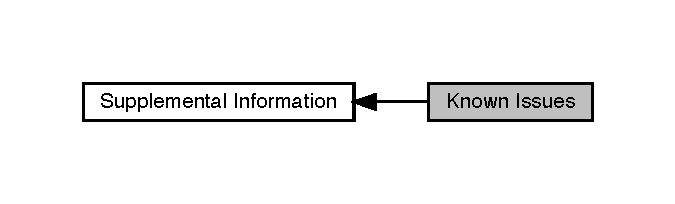
\includegraphics[width=324pt]{a00846}
\end{center}
\end{figure}
